\documentclass[conference,a4paper]{IEEEtran}

% Escritura mejorada de fórmulas matemáticas
\usepackage{amsmath}

% Inserción de gráficos
\usepackage{graphicx}

% Escritura de pseudocódigo
\usepackage[kw]{pseudo}

% Escritura mejorada de tablas
\usepackage{booktabs}

% Escritura mejorada de citas bibliográficas
\usepackage{cite}


% Macros traducidas
\def\contentsname{Índice general}
\def\listfigurename{Índice de figuras}
\def\listtablename{Índice de tablas}
\def\refname{Referencias}
\def\indexname{Índice alfabético}
\def\figurename{Fig.}
\def\tablename{TABLA}
\def\partname{Parte}
\def\appendixname{Apéndice}
\def\abstractname{Resumen}
% IEEE specific names
\def\IEEEkeywordsname{Palabras clave}
\def\IEEEproofname{Demostración}


\begin{document}

\title{Ensamble Secuencial de Modelos para predicción de precios de vivienda y enfermedad de Parkinson}

\author{
  \IEEEauthorblockN{Joaquín Borja León}
  \IEEEauthorblockA{
    \textit{Dpto. Ciencias de la Computación e Inteligencia Artificial}\\
    \textit{Universidad de Sevilla}\\
    Sevilla, España\\
    joaborleo@alum.us.es}
  
  \and
  
  \IEEEauthorblockN{Héctor Guerra Prada}
  \IEEEauthorblockA{
    \textit{Dpto. Ciencias de la Computación e Inteligencia Artificial}\\
    \textit{Universidad de Sevilla}\\
    Sevilla, España\\
    hecguepra@alum.us.es}
}

\maketitle


% Resumen
\begin{abstract}
Este trabajo presenta la implementación desde cero de un meta-algoritmo de ensamble secuencial para tareas de regresión. Se utilizan dos estimadores débiles: \texttt{DecisionTreeRegressor} y \texttt{LinearRegression}. Se aplican ambos enfoques a dos conjuntos de datos: precios de viviendas (\texttt{house\_prices.csv}) y datos clínicos de la enfermedad de Parkinson (\texttt{parkinsons.csv}). La búsqueda manual de hiperparámetros se realiza mediante validación cruzada, optimizando \texttt{n\_estimators}, \texttt{sample\_size}, \texttt{lr}, \texttt{max\_depth} para árboles y \texttt{fit\_intercept} para regresión lineal. También se incluye un mecanismo opcional de parada temprana (\emph{early stopping}). Los resultados demuestran que \texttt{DecisionTreeRegressor} capta relaciones no lineales en Parkinson (R²=0.9323) y \texttt{LinearRegression} funciona bien en precios de vivienda (R²=0.7875).
\end{abstract}


% Palabras claves
\begin{IEEEkeywords}
  Inteligencia Artificial, Ensamble Secuencial, Regresión, Boosting, Precios de Vivienda, Enfermedad de Parkinson.
\end{IEEEkeywords}

%SECCIÓN INTRODUCCIÓN
\section{Introducción}

Los métodos basados en ensambles han demostrado una capacidad predictiva superior a la de modelos individuales en múltiples dominios. En particular, los ensambles secuenciales construyen modelos débiles de forma iterativa, de modo que cada nuevo estimador corrige los errores residuales del conjunto previo. Este esquema es la base de algoritmos como AdaBoost y Gradient Boosting \cite{freund1997decision, friedman2001elements}.

El objetivo de este trabajo es implementar y estudiar un meta-algoritmo de ensamble secuencial para tareas de regresión, aplicándolo a dos conjuntos de datos con características muy distintas:
\begin{itemize}
    \item Conjunto de datos de precios de viviendas (\texttt{house\_prices.csv}): 560 registros con variables físicas y categóricas, prediciendo el precio de venta.
    \item Conjunto de datos de la enfermedad de Parkinson (\texttt{parkinsons.csv}): 2000 registros con datos clínicos y de señal de voz, prediciendo la puntuación total del UPDRS.
\end{itemize}

La métrica principal de evaluación es el coeficiente de determinación (R²), complementado con el error absoluto medio (MAE). Los objetivos específicos son:
\begin{enumerate}
    \item Implementar las fases de entrenamiento y predicción del ensamble secuencial sin usar librerías de boosting de alto nivel.
    \item Comparar dos estimadores débiles: \texttt{DecisionTreeRegressor} y \texttt{LinearRegression}.
    \item Realizar búsqueda manual de hiperparámetros (\texttt{n\_estimators}, \texttt{sample\_size}, \texttt{lr}, \texttt{max\_depth} para árboles y \texttt{fit\_intercept} para lineal) mediante validación cruzada.
    \item Implementar un mecanismo opcional de \emph{early stopping} basado en un subconjunto de validación interno.
    \item Documentar todas las decisiones de diseño, exponer resultados reproducibles y extraer conclusiones.
\end{enumerate}

La estructura del documento es la siguiente:
\begin{itemize}
    \item Sección II: Preliminares.
    \item Sección III: Metodología.
    \item Sección IV: Resultados.
    \item Sección V: Conclusiones.
    \item Referencias bibliográficas.
\end{itemize}

%SECCIÓN PRELIMINARES
\section{Preliminares}
\subsection{Métodos empleados}
En este trabajo se utiliza el enfoque de ensamble secuencial (boosting). Cada estimador débil se entrena sobre los residuos del conjunto acumulado anterior. La función de pérdida es el error cuadrático medio, de modo que el residuo en la iteración \(m\) es:
\begin{equation}
r_{im} = y_i - F_{m-1}(x_i).
\end{equation}

Se consideran dos familias de estimadores débiles:
\begin{enumerate}
    \item \texttt{DecisionTreeRegressor} (árbol de decisión) con profundidad máxima (\texttt{max\_depth}) variable.
    \item \texttt{LinearRegression} (regresión lineal).
\end{enumerate}

\subsection{Trabajo relacionado}
Los ensambles de boosting (AdaBoost, Gradient Boosting, XGBoost) han sido ampliamente estudiados en literatura reciente \cite{freund1997decision, friedman2001elements, chen2016xgboost}. A diferencia de nuestro enfoque, se suele utilizar implementaciones optimizadas de alto nivel. En este trabajo implementamos desde cero la lógica de boosting.


%SECCIÓN METODOLOGÍA
\section{Metodología}
En esta sección se describe el algoritmo de ensamble secuencial implementado. La implementación sigue el siguiente esquema:

\begin{figure}[h]
    \centering
    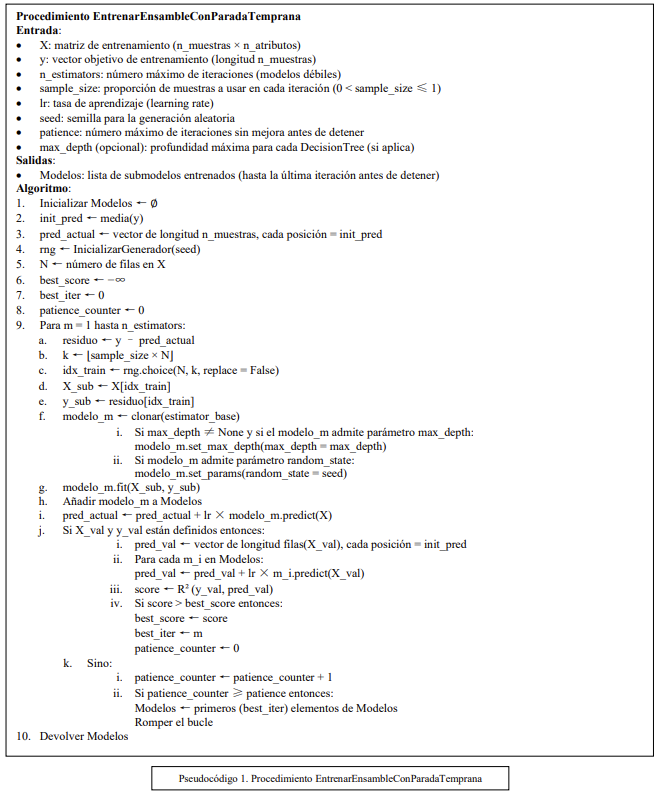
\includegraphics[width=0.5\textwidth]{early.png}
    \caption{}
    \label{fig:1}
\end{figure}

\begin{figure}[h]
    \centering
    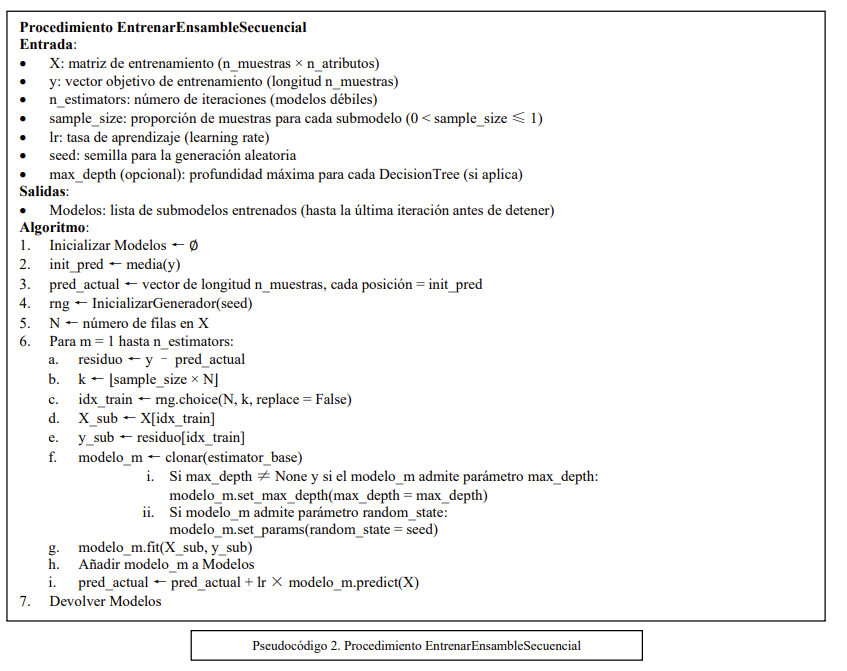
\includegraphics[width=0.5\textwidth]{Sin early.png}
    \caption{}
    \label{fig:2}
\end{figure}

\begin{figure}[h]
    \centering
    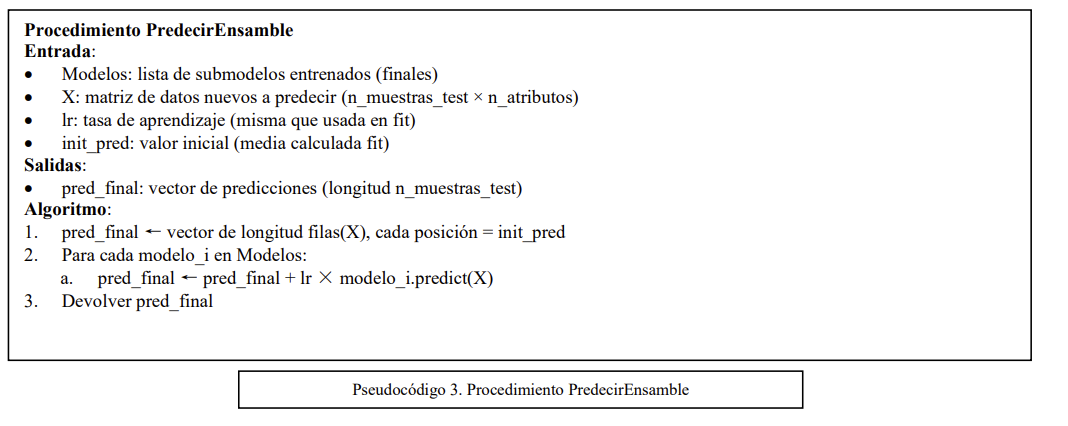
\includegraphics[width=0.5\textwidth]{Predict.png}
    \caption{}
    \label{fig:3}
\end{figure}

\subsubsection*{Modelos base: DecisionTreeRegressor, LinearRegression y Early Stopping}

\paragraph{DecisionTreeRegressor} 
El \texttt{DecisionTreeRegressor} es un modelo de aprendizaje supervisado que predice valores numéricos dividiendo el espacio de características en regiones, siguiendo una estructura jerárquica en forma de árbol. En cada nodo, se elige la variable y el umbral que mejor separen los datos para minimizar el error de predicción. Es un modelo \emph{no lineal}, capaz de capturar relaciones complejas entre variables, aunque puede sobreajustar si no se controla su profundidad.

\paragraph{LinearRegression} 
El modelo \texttt{LinearRegression} ajusta una función lineal a los datos, minimizando el error cuadrático medio entre las predicciones y los valores reales. Es un modelo \emph{lineal y simple}, adecuado cuando hay una relación aproximadamente lineal entre las variables predictoras y la variable objetivo. No capta relaciones no lineales ni interacciones, pero tiene bajo riesgo de sobreajuste y es computacionalmente eficiente.

\paragraph{Early Stopping} 
Para implementar el mecanismo de \emph{early stopping}, en cada iteración se reserva un 20\% del conjunto de entrenamiento (subconjunto de validación). Se calcula el error en validación después de cada nuevo modelo y se detiene el entrenamiento si no hay mejora tras \texttt{patience} iteraciones consecutivas.

\section{Resultados}
\subsection{Ensamble con DecisionTreeRegressor}
Configuración de partida: \texttt{DecisionTreeRegressor(max\_depth=3)}, \texttt{n\_estimators=50}, \texttt{sample\_size=0.8}, \texttt{lr=0.1}, \texttt{random\_state=42}. Validación cruzada 5-fold:
\begin{itemize}
    \item \textbf{House Prices}: R² por fold = [0.72356832 0.75864956 0.76608286 0.78143207 0.77203406], media = 0.7603533739391801.
    \item \textbf{Parkinsons}: R² por fold = [0.63276246 0.66040138 0.63794864 0.65623765 0.6812172], media = 0.6537134652991631.
\end{itemize}

Primera búsqueda manual de hiperparámetros (Grid Search simple):
\[
\begin{aligned}
& n\_estimators \in \{10, 50, 100\}, \\
& lr \in \{0.01, 0.1, 0.2\}, \\
& sample\_size \in \{0.6, 0.8, 1.0\}, \\
& max\_depth \in \{3, 5, 7\}.
\end{aligned}
\]
\begin{table}[h]
\centering
\caption{Top-10 House Prices – Primera búsqueda}
\begin{tabular}{|c|c|c|c|c|}
\hline
$n\_estimators$ & $lr$ & $sample\_size$ & $max\_depth$ & $r^2\_mean$ \\
\hline
100 & 0.2 & 0.8 & 3 & 0.790717 \\
100 & 0.1 & 0.6 & 3 & 0.790011 \\
100 & 0.2 & 1.0 & 3 & 0.788360 \\
\hline
\end{tabular}
\end{table}


\begin{table}[h]
\centering
\caption{Top-10 Parkinsons – Primera búsqueda}
\begin{tabular}{|c|c|c|c|c|}
\hline
$n\_estimators$ & $lr$ & $sample\_size$ & $max\_depth$ & $r^2\_mean$ \\
\hline
100 & 0.1 & 1.0 & 7 & 0.919854 \\
100 & 0.2 & 1.0 & 7 & 0.916761 \\
50 & 0.2 & 1.0 & 7 & 0.915149 \\
\hline
\end{tabular}
\end{table}


Evaluación final en test:
\begin{itemize}
    \item \textbf{House Prices (óptimo):} $n\_estimators=150$, $lr=0.3$, $sample\_size=1.0$, $max\_depth=3$. \\ Test R² = 0.7191232968866706, MAE = 29074.149712968017.
    \item \textbf{Parkinsons (óptimo):} $n\_estimators=100$, $lr=0.1$, $sample\_size=1.0$, $max\_depth=7$. \\ Test R² =  0.936545781009529, MAE = 1.615012580924182.
\end{itemize}

\subsection{Ensamble con LinearRegression}
Configuración inicial: \texttt{LinearRegression
(fit\_intercept=True)}, \texttt{n\_estimators=50}, \texttt{sample\_size=0.8}, \texttt{lr=0.1}, \texttt{random\_state=42}. Validación cruzada 5-fold:
\begin{itemize}
    \item \textbf{House Prices}: R² por fold = [0.60978187 0.77420332 0.65521267 0.82114321 0.44958941], media = 0.6619860969721221.
    \item \textbf{Parkinsons}: R² por fold = [0.20806173 0.2282059  0.12500756 0.12577325 0.1387287], media = 0.16515542749688544.
\end{itemize}

Primera búsqueda manual de hiperparámetros:
\[
\begin{aligned}
& n\_estimators \in \{10, 50, 100\}, \\
& lr \in \{0.01, 0.1, 0.2\}, \\
& sample\_size \in \{0.6, 0.8, 1.0\}, \\
& fit\_intercept \in \{\text{True}, \text{False}\}.
\end{aligned}
\]
\begin{table}[h]
\centering
\caption{Top-5 House Prices – Primera búsqueda}
\begin{tabular}{|c|c|c|c|c|}
\hline
$n\_estimators$ & $lr$ & $sample\_size$ & $fit\_intercept$ & $r^2\_mean$ \\
\hline
10 & 0.2 & 1.0 & True & 0.720497 \\
10 & 0.2 & 0.8 & True  & 0.715898 \\
50 & 0.1 & 1.0 & True & 0.703330 \\
\hline
\end{tabular}
\end{table}


\begin{table}[h]
\centering
\caption{Top-5 Parkinsons – Primera búsqueda}
\begin{tabular}{|c|c|c|c|c|}
\hline
$n\_estimators$ & $lr$ & $sample\_size$ & $fit\_intercept$ & $r^2\_mean$ \\
\hline
10 & 0.2 & 1.0 & True & 0.166249 \\
10 & 0.2 & 0.8 & True & 0.166206 \\
50 & 0.2 & 0.8 & True & 0.166206 \\
\hline
\end{tabular}
\end{table}


Evaluación final en test:
\begin{itemize}
    \item \textbf{House Prices (lineal óptimo):} $n\_estimators=10$, $lr=0.2$, $sample\_size=1.0$, $fit\_intercept=True$. \\ Test R² = 0.766222639788844, MAE = 25257.28627191641.
    \item \textbf{Parkinsons (lineal óptimo):} $n\_estimators=10$, $lr=0.2$, $sample\_size=1.0$, $fit\_intercept=True$. \\ Test R² = 0.14895427840774145, MAE = 8.073492674590106.
\end{itemize}

\subsection{Early Stopping (Parada Temprana)}
\begin{itemize}
    \item \textbf{House (LR + early stopping):} Test R² = 0.766222639788844, MAE = 25257.28627191643.
    \item \textbf{Parkinsons (LR + early stopping):} Test R² = 0.14887395829827899, MAE = 8.077265793598144.
\end{itemize}

\section{Conclusiones}
\begin{itemize}
    
    \item Este trabajo ha abordado la implementación desde cero de un meta-algoritmo de ensamble secuencial para tareas de regresión, aplicándolo a dos conjuntos de datos de naturaleza diferente: precios de viviendas y progresión de la enfermedad de Parkinson. Se han comparado dos tipos de modelos base (\texttt{DecisionTreeRegressor} y \texttt{LinearRegression}) y se ha evaluado su rendimiento mediante validación cruzada y métricas como el coeficiente de determinación ($R^2$) y el error absoluto medio (MAE). Asimismo, se ha incorporado un mecanismo de parada temprana para optimizar el proceso de entrenamiento.

   \item Los resultados muestran que el desempeño del meta-modelo depende en gran medida del tipo de estimador base utilizado. El modelo basado en árboles obtuvo un rendimiento excelente en el conjunto de Parkinson ($R^2 = 0.936545781009529$), gracias a su capacidad para capturar relaciones no lineales complejas. En cambio, su rendimiento fue inferior en el conjunto de precios de vivienda, donde alcanzó $R^2 = 0.678402654711951$, posiblemente debido al tamaño limitado del dataset, que restringe la capacidad de generalización del ensamble. Por otro lado, la regresión lineal se comportó mejor en este conjunto ($R^2 = 0.766222639788844$), mostrando mayor estabilidad con pocos datos y relaciones más simples. Sin embargo, en el conjunto de Parkinson, su desempeño fue muy bajo ($R^2 = 0.14895427840774145$), debido a que los valores no siguen una relación lineal clara con las variables predictoras. La búsqueda manual de hiperparámetros permitió identificar configuraciones óptimas en ambos casos.

\end{itemize}

\begin{thebibliography}{1}
\bibitem{freund1997decision}
Y.~Freund and R.~Schapire, ``A Decision-Theoretic Generalization of On-Line Learning and an application to boosting,'' \emph{Journal of Computer and System Sciences}, 1997.

\bibitem{friedman2001elements}
J.~Friedman, T.~Hastie, and R.~Tibshirani, ``The Elements of Statistical Learning,'' Springer, 2001.

\bibitem{chen2016xgboost}
T.~Chen and C.~Guestrin, ``XGBoost: A Scalable Tree Boosting System,'' in \emph{Proceedings of the 22nd ACM SIGKDD International Conference on Knowledge Discovery and Data Mining}, 2016.

\bibitem{sklearn_linear}
Scikit-learn Developers, ``LinearRegression,'' \emph{https://scikit-learn.org/stable/modules/generated/sklearn.linear\_model.LinearRegression.html}.

\bibitem{sklearn_tree}
Scikit-learn Developers, ``DecisionTreeRegressor,'' \emph{https://scikit-learn.org/stable/modules/generated/sklearn.tree.DecisionTreeRegressor.html}.
\end{thebibliography}

\end{document}
